%%%%%%%%%%%%%%%%%%%%%%%%%%%%%%%%%%%%%%%%%%%%%%%%%%%%%%%%%%%%%%%%%%%%%%%%%%%%%%%%
% Medium Length Graduate Curriculum Vitae
% LaTeX Template
% Version 1.2 (3/28/15)
%
% This template has been downloaded from:
% http://www.LaTeXTemplates.com
%
% Original author:
% Rensselaer Polytechnic Institute 
% (http://www.rpi.edu/dept/arc/training/latex/resumes/)
%
% Modified by:
% Daniel L Marks <xleafr@gmail.com> 3/28/2015
%
% Important note:
% This template requires the res.cls file to be in the same directory as the
% .tex file. The res.cls file provides the resume style used for structuring the
% document.
%
%%%%%%%%%%%%%%%%%%%%%%%%%%%%%%%%%%%%%%%%%%%%%%%%%%%%%%%%%%%%%%%%%%%%%%%%%%%%%%%%

%-------------------------------------------------------------------------------
%	PACKAGES AND OTHER DOCUMENT CONFIGURATIONS
%-------------------------------------------------------------------------------

%%%%%%%%%%%%%%%%%%%%%%%%%%%%%%%%%%%%%%%%%%%%%%%%%%%%%%%%%%%%%%%%%%%%%%%%%%%%%%%%
% You can have multiple style options the legal options ones are:
%
%   centered:	the name and address are centered at the top of the page 
%				(default)
%
%   line:		the name is the left with a horizontal line then the address to
%				the right
%
%   overlapped:	the section titles overlap the body text (default)
%
%   margin:		the section titles are to the left of the body text
%		
%   11pt:		use 11 point fonts instead of 10 point fonts
%
%   12pt:		use 12 point fonts instead of 10 point fonts
%
%%%%%%%%%%%%%%%%%%%%%%%%%%%%%%%%%%%%%%%%%%%%%%%%%%%%%%%%%%%%%%%%%%%%%%%%%%%%%%%%

\documentclass[margin]{res}  

% Default font is the helvetica postscript font
\usepackage{helvet}

% Increase text height
\textheight=700pt

\usepackage{graphicx}
\usepackage{multirow}

\begin{document}

%-------------------------------------------------------------------------------
%	NAME AND ADDRESS SECTION
%-------------------------------------------------------------------------------
\name{TITHI FLORENCE D'COSTA}

% Note that addresses can be used for other contact information:
% -phone numbers
% -email addresses
% -linked-in profile

% Simulate as if there are 7 lines of address
\address{\\84/2 Kakrail, Ramna, Dhaka-1000\\Mobile: 01914296808
\\Phone: 0088029357638
\\Email: dcosta.florence@yahoo.com}
% Hence the photo would take 7 lines/rows
%\address{\multirow{7}{*}{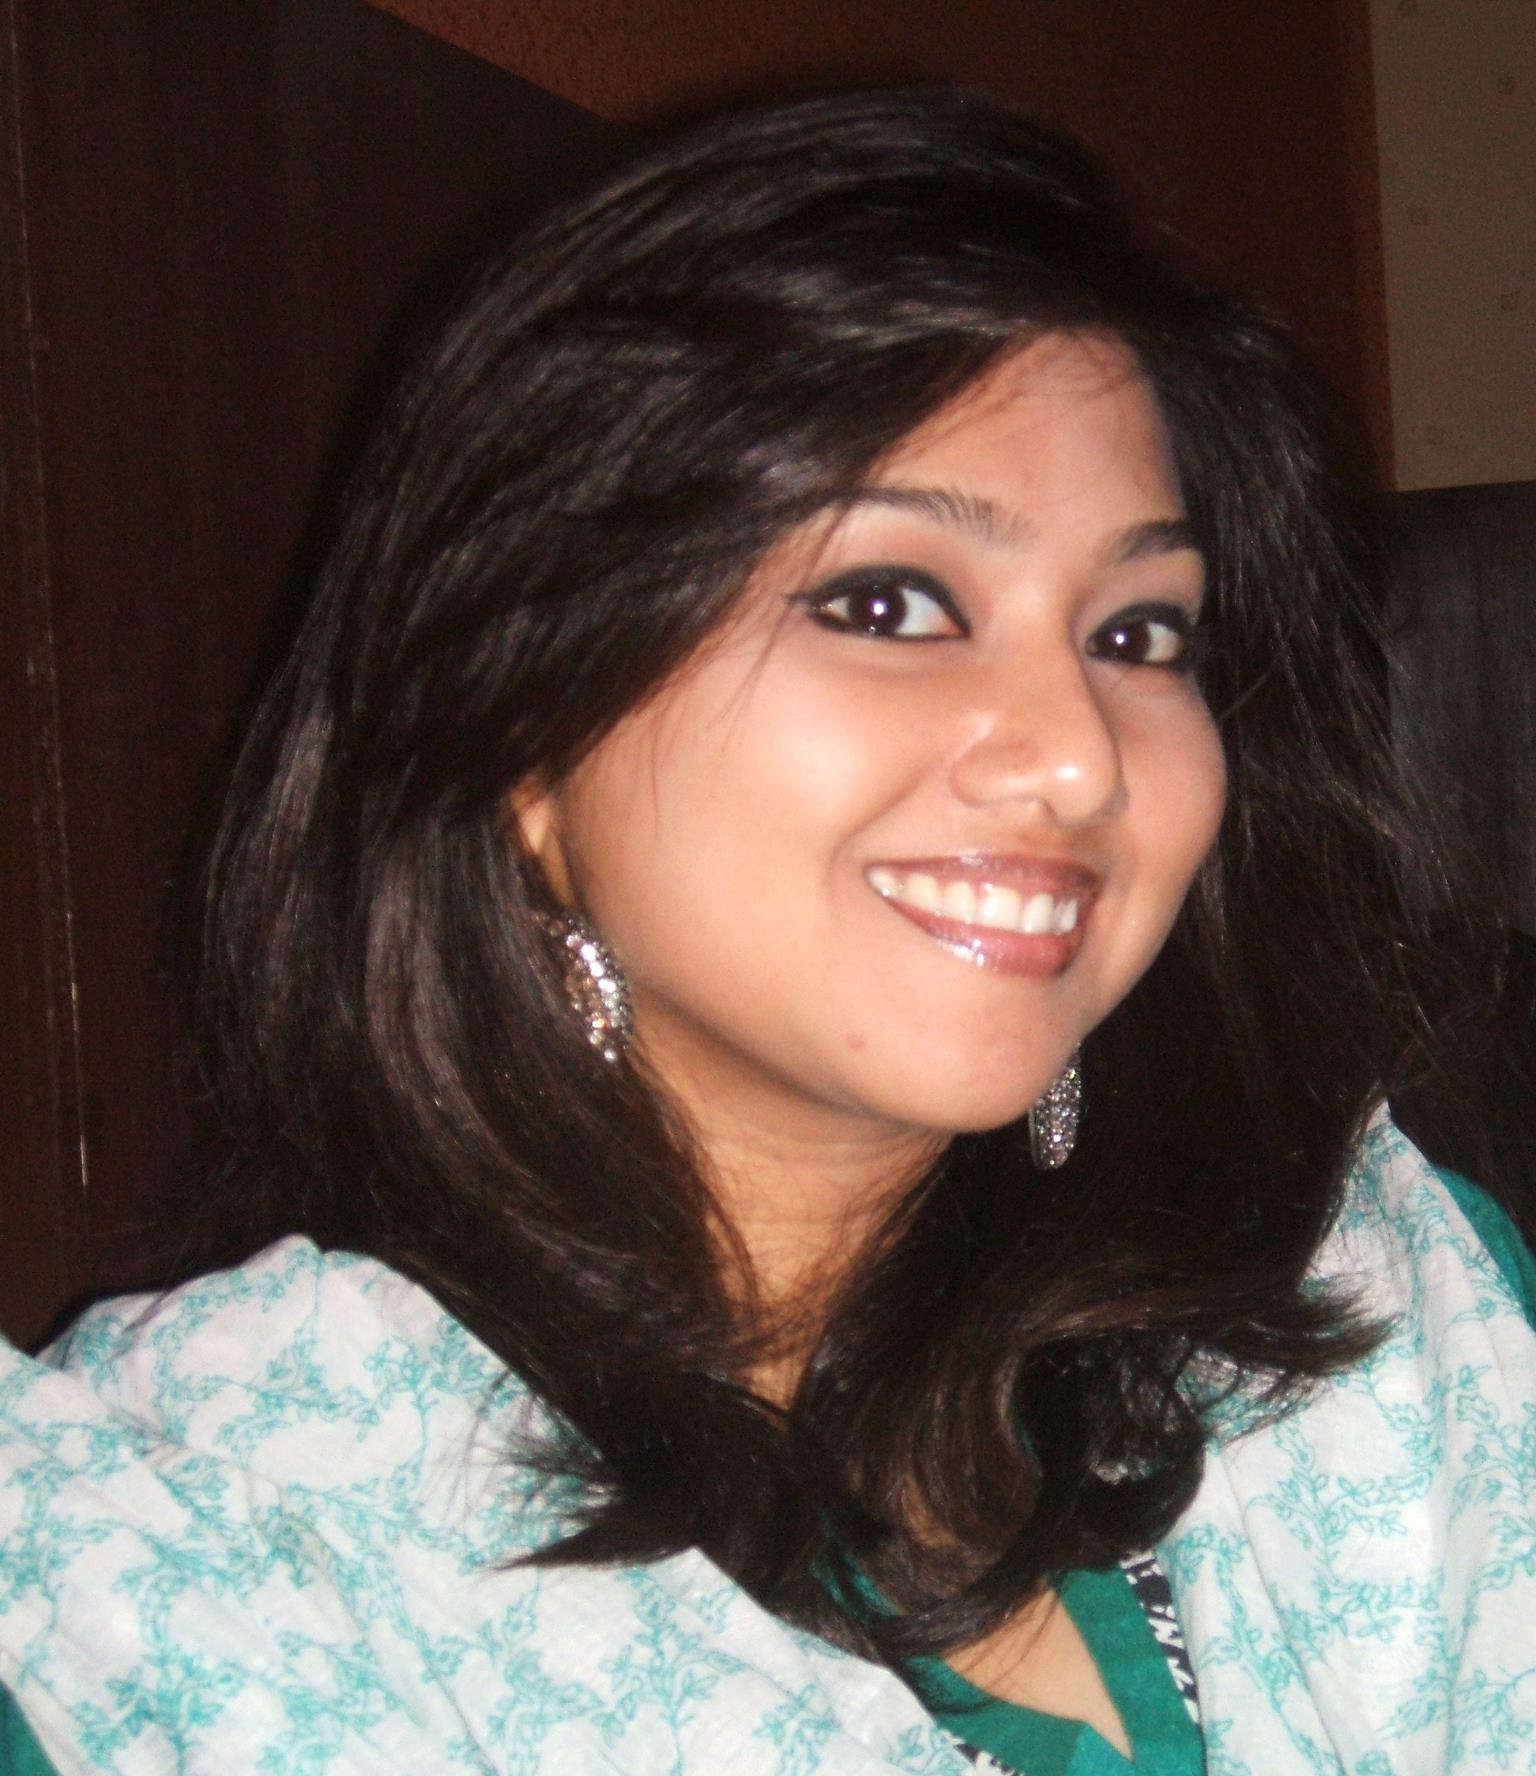
\includegraphics[width=2.7cm, height=2.9cm]{1}}}

% Uncomment to add a third address
%\address{Address 3 line 1\\Address 3 line 2\\Address 3 line 3}
%-------------------------------------------------------------------------------

\begin{resume}
%-------------------------------------------------------------------------------
%	CAREER OBJECTIVE
%-------------------------------------------------------------------------------
%
\section{CAREER OBJECTIVE}
\par
To build my career in a teaching profession, where I can get the opportunities to prove my abilities by accepting challenges, fulfilling the organizational goal and climb the career ladder through continuous learning and commitment. I would like utilize my lively and energetic attitude in teaching students with great enthusiasm. I would also like to offer quality education to students.

%-------------------------------------------------------------------------------


%-------------------------------------------------------------------------------
%	EDUCATION SECTION
%-------------------------------------------------------------------------------
\section{EDUCATION}
\textbf{Heriot Watt University(UK)}\\
{\sl BBA (Bachelor of Business Administration)}, June 2015\hfill Result: 
1st Class
\\ \\
\textbf{Scottish Qualification Authority(UK)}\\
{\sl Higher Diploma in Accounting}, February 2013 
\\ \\
\textbf{Dhaka City College}\\
{\sl Higher Secondary Certificate (HSC)}, 2006 \hfill G.P.A- 4.5 out of 5
\\ \\
\textbf{Holy Cross Girls' High School}\\
{\sl Secondary School Certificate (SSC)}, 2004 \hfill G.P.A- 4.63 out of 5

%-------------------------------------------------------------------------------

%-------------------------------------------------------------------------------
%	PROJECTS SECTION
%-------------------------------------------------------------------------------
%%
%\section{PROJECTS}
%\par
%\textbf{Project One}: 
%Lorem ipsum dolor sit amet, consectetur adipiscing elit. Pellentesque semper 

%-------------------------------------------------------------------------------


%-------------------------------------------------------------------------------
%	EXPERIENCE SECTION
%-------------------------------------------------------------------------------
% Modify the format of each position
\begin{format}
\title{l}\employer{r}\\
\dates{l}\location{r}\\
\body\\
\end{format}
%-------------------------------------------------------------------------------

\section{EXPERIENCE}

\employer{Primark Store Ltd.}
\location{499-517 Oxford St, London W1K 7DA, UK}
\dates{04/2010- 09/2011}
\title{\textbf{Retail operative}}
\begin{position}
\textbf{Skill Achieved:}
Customer service, Stock Management, Team work, Task Allocation, Supervision, Records Management, Cash Handling, Transaction Process, Write weekly Report.
\end{position}

\employer{St. Merry's Youth Organization}
\location{Ramna Church, Dhaka}
\dates{01/2007- 12/2009}
\title{\textbf{General Secretary}}
\begin{position}
\textbf{Responsibilities:}
Writing minutes and agendas, issuing letter for committee members, organizing educational and cultural programs, arranging monthly meeting, email handling, editorial job for yearly publication, maintaining files for official correspondence.
\end{position}

\textbf{House Teacher:} Teaching experience class KG to class 8 as private tutor both english and bangla medium.

% \textbf{Secretary:}  Working as a secretary of St. Merry's Youth Organization, Ramna Church, Dhaka.\\
% \textbf{Responsibilities:} Writing minutes and agendas, issuing letter for committee members, organizing educational and cultural programs, arranging monthly meeting.
  
%-------------------------------------------------------------------------------
%	COMPUTER SKILLS SECTION
%-------------------------------------------------------------------------------
\section{SKILLS}

\textbf{Technical skills:} Microsoft word, Microsoft Excel, Power point, Email handling, report writing.
\\
\textbf{Personal Skills:} High level of concentration, Accurate keyboard skills, sound judgment, honesty, integrity, professional appearance, strong numerical skill.
\\
\textbf{Language Skills:} English (good at writing and speaking). IELTS SCORE: 6
%-------------------------------------------------------------------------------


%-------------------------------------------------------------------------------
%	PERSONAL PROFILE
%-------------------------------------------------------------------------------
\section{PERSONAL PROFILE}
\textbf{Father's Name:}: Peter B. D'costa 
\\
\textbf{Date of Birth:} 3rd August 1987
\\
\textbf{Marital Status:} Married
%-------------------------------------------------------------------------------


%-------------------------------------------------------------------------------
%	Interests
%-------------------------------------------------------------------------------
\section{INTERESTS}
Watching movie and documentary, Internet Browsing.
%-------------------------------------------------------------------------------


%-------------------------------------------------------------------------------
%	References
%-------------------------------------------------------------------------------
\section{REFERENCES}
References are available upon request.
%-------------------------------------------------------------------------------

\end{resume}
\end{document}